%% https://stackoverflow.com/questions/1603301/how-to-add-page-numbers-to-postscript-pdf

%\documentclass[8pt]{article}
\documentclass{article}
%\usepackage[final]{pdfpages}
\usepackage{pdfpages}
\usepackage{fancyhdr}

%% original
%\topmargin 70pt
%\oddsidemargin 70pt

%% letter size
%\topmargin -70pt
%\oddsidemargin 170pt

%% beamer
%% needs trial and error
\topmargin -425pt
\oddsidemargin -64pt

\pagestyle{fancy}
\rfoot{\Large\thepage}
\cfoot{}
%\renewcommand {\headrulewidth}{10pt}
%\renewcommand {\footrulewidth}{10pt}
\renewcommand {\headrulewidth}{0pt}
\renewcommand {\footrulewidth}{0pt}

%% https://tex.stackexchange.com/questions/2095/what-is-the-simplest-way-to-typeset-an-entire-document-in-sans-serif
\renewcommand{\familydefault}{\sfdefault}

\begin{document}
\includepdfset{pagecommand=\thispagestyle{fancy}}
%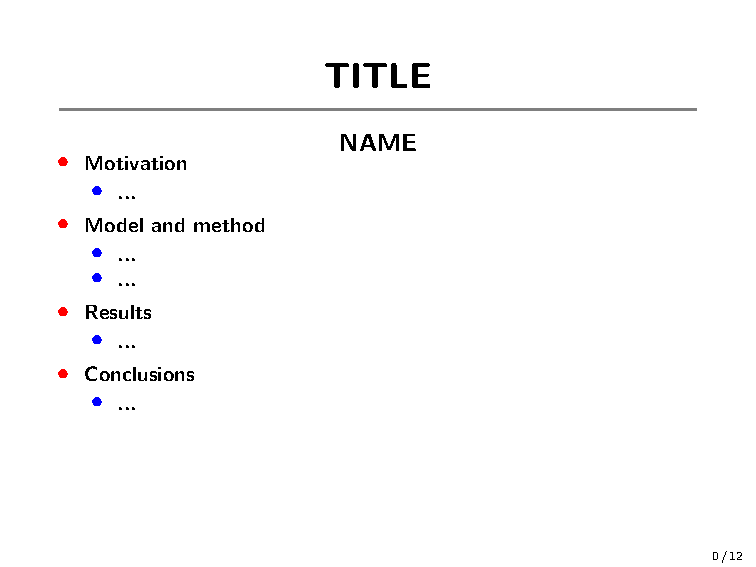
\includepdf[fitpaper=true,scale=0.98,pages=-]{_slide.pdf} %% original
%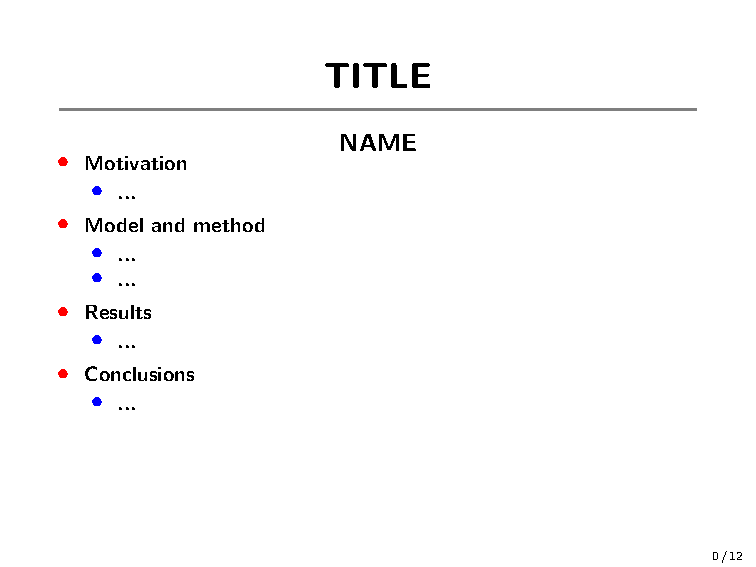
\includepdf[pages=-]{_slide.pdf} %% letter size
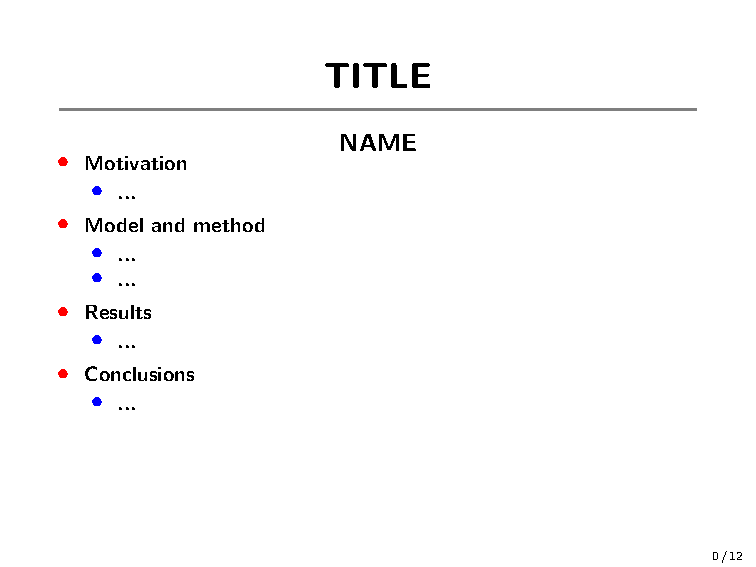
\includepdf[fitpaper=true,pages=-]{_slide.pdf} %% beamer
% fitpaper & scale aren't always necessary - depends on the paper being submitted.
\end{document}
